
% VLDB template version of 2020-08-03 enhances the ACM template, version 1.7.0:
% https://www.acm.org/publications/proceedings-template
% The ACM Latex guide provides further information about the ACM template

\documentclass[sigconf, nonacm]{acmart}
\usepackage{booktabs}

%% The following content must be adapted for the final version
% paper-specific
\newcommand\vldbdoi{XX.XX/XXX.XX}
\newcommand\vldbpages{XXX-XXX}
% issue-specific
\newcommand\vldbvolume{14}
\newcommand\vldbissue{1}
\newcommand\vldbyear{2020}
% should be fine as it is
\newcommand\vldbauthors{\authors}
\newcommand\vldbtitle{\shorttitle}
% leave empty if no availability url should be set
\newcommand\vldbavailabilityurl{}
% whether page numbers should be shown or not, use 'plain' for review versions, 'empty' for camera ready
\newcommand\vldbpagestyle{plain}

\begin{document}
\title{Unite! Researcher's Search: A Multi-Source Engine for Interdisciplinary Research Collaboration}

\author{Łukasz Augustyniak}
\affiliation{\institution{Wroclaw University of Science and Technology}}
\email{lukasz.augustyniak@pwr.edu.pl}

\author{Paweł Litwin}
\affiliation{\institution{Wroclaw University of Science and Technology}}
\email{290374@student.pwr.edu.pl}

\author{Iwo Smura}
\affiliation{\institution{Wroclaw University of Science and Technology}}
\email{iwo.smura@student.pwr.edu.pl}

\author{Julia Farganus}
\affiliation{\institution{Wroclaw University of Science and Technology}}
\email{julia.farganus@student.pwr.edu.pl}

\author{Kamil Tagowski}
\affiliation{\institution{Wroclaw University of Science and Technology}}
\email{kamil.tagowski@pwr.edu.pl}

\author{Tomasz Kajdanowicz}
\affiliation{\institution{Wroclaw University of Science and Technology}}
\email{tomasz.kajdanowicz@pwr.edu.pl}

\begin{abstract}
Discovering potential collaborators across disciplinary and institutional boundaries remains a persistent challenge in academia: existing platforms suffer from fragmented author profiles, incomplete institutional metadata, and the absence of unified cross-platform search with direct contact information.
We present \textsc{Unite! Researcher's Search}, a researcher discovery engine developed within the Unite! European University Alliance that fuses bibliographic data from OpenAlex, verified identities from ORCID, and publication metadata from Crossref into enriched researcher profiles spanning nine European universities.
The system integrates a hybrid retrieval architecture that combines semantic vector search with keyword matching over nearly 3M publications and 213K researcher profiles, enabling both exploratory and precise queries.
In this demonstration, attendees interact with the system through live queries---searching for collaborators by research topic, exploring multi-source enriched profiles with verified contact information, and performing audience-driven free-form searches that showcase the system's flexibility and real-time responsiveness.
\end{abstract}

\maketitle

%%% do not modify the following VLDB block %%
%%% VLDB block start %%%
\pagestyle{\vldbpagestyle}
\begingroup\small\noindent\raggedright\textbf{PVLDB Reference Format:}\\
\vldbauthors. \vldbtitle. PVLDB, \vldbvolume(\vldbissue): \vldbpages, \vldbyear.\\
\href{https://doi.org/\vldbdoi}{doi:\vldbdoi}
\endgroup
\begingroup
\renewcommand\thefootnote{}\footnote{\noindent
This work is licensed under the Creative Commons BY-NC-ND 4.0 International License. Visit \url{https://creativecommons.org/licenses/by-nc-nd/4.0/} to view a copy of this license. For any use beyond those covered by this license, obtain permission by emailing \href{mailto:info@vldb.org}{info@vldb.org}. Copyright is held by the owner/author(s). Publication rights licensed to the VLDB Endowment. \\
\raggedright Proceedings of the VLDB Endowment, Vol. \vldbvolume, No. \vldbissue\ %
ISSN 2150-8097. \\
\href{https://doi.org/\vldbdoi}{doi:\vldbdoi} \\
}\addtocounter{footnote}{-1}\endgroup
%%% VLDB block end %%%

%%% do not modify the following VLDB block %%
%%% VLDB block start %%%
\ifdefempty{\vldbavailabilityurl}{}{
\vspace{.3cm}
\begingroup\small\noindent\raggedright\textbf{PVLDB Artifact Availability:}\\
The source code, data, and/or other artifacts have been made available at \url{\vldbavailabilityurl}.
\endgroup
}
%%% VLDB block end %%%

\section{Introduction}
% ~0.8 pages
%
% Motivation: finding interdisciplinary research collaborators is hard
% - researchers are siloed within their domains
% - existing tools (Scopus, SciVal, Google Scholar, Semantic Scholar, OpenAlex, ResearchGate)
%   have limitations for cross-domain discovery
%
% Limitations of existing tools (inline, no separate Related Work):
% - Scopus/SciVal: proprietary, expensive, limited API
% - Google Scholar: no structured data, no API
% - Semantic Scholar/OpenAlex: good APIs but no researcher-centric search for collaboration
% - ResearchGate: social network, not a search engine
%
% Comparison table or inline comparison showing what Unite enables vs others
% (this is the "novelty and significance" the CFP asks for)
%
% Unite solution overview (1-2 sentences):
% - integrates multiple open data sources into a unified researcher search engine
% - enriches researcher/paper profiles with data from ORCID, DOI, heuristic email extraction
%
% Contributions (3-4 bullets):
% \begin{itemize}
%   \item A data integration pipeline merging OpenAlex + Semantic Scholar
%   \item An enrichment framework combining ORCID, DOI, and heuristic methods
%   \item An interactive search interface for interdisciplinary collaborator discovery
%   \item A demonstration comparing Unite's capabilities against existing tools
% \end{itemize}


% The landscape of academic discovery is currently dominated by several large-scale platforms.
% Within this ecosystem, Google Scholar offers the largest index (~400M publications).
% Its search is primarily keyword-based and supports only a limited set of filters, which can constrain more nuanced queries.
% It suffers from inconsistent researcher profiles as these are optional and the platform lacks ORCID integration.
% OpenAlex is an open bibliographic database (~240M publications, 100M authors) that uses ORCID as its primary author identifier, supplemented by machine-learning–based disambiguation.
% While this approach improves coverage, it still leads to issues such as profile fragmentation or the merging of records for authors with similar names.
% In addition, institution metadata remains limited, and affiliation-based search is relatively underdeveloped. Search is mainly key-word based, with semantic search being under development.
% Scopus, a subscription-based citation database (~100M publications, 21.9M profiles), provides more advanced AI-driven functionality, including well-developed author and affiliation search. However, its reliance on costly institutional subscriptions makes it impractical as a data source for open or independently funded projects.
% Semantic Scholar (~225M papers, 79M authors) offers a free REST API, making it a useful supplementary data source. It includes AI-powered features such as semantic search and automated summaries, with author disambiguation model [cite]. Despite these strengths, the platform still suffers from profile fragmentation, where a single researcher’s work may be split across multiple incomplete or unverified profiles, and it lacks robust institution-level search.
% ResearchGate functions primarily as a social network (~160M publications, 25M users), facilitating direct interaction between researchers, including messaging and paper requests. However, much of its content is self-uploaded and not formally verified, and it's intrusive email and notification practices can discourage collaboration engagement.
% Several additional tools—such as ResearchRabbit, Connected Papers, and Consensus—support literature exploration, though none serve as comprehensive, standalone primary databases.

Identifying potential research collaborators outside one's own discipline or institution is a critical yet largely unsolved challenge. Researchers typically rely on personal networks or keyword searches within siloed platforms, each covering only a fragment of the global scholarly record. This gap is felt acutely not only by researchers themselves but also by university units responsible for bridging academia and industry---such as technology transfer offices and innovation centers---which currently lack dedicated tools for searching and matching researchers to external partners. While a diverse ecosystem of tools has emerged to support literature discovery and researcher profiling, their effectiveness is constrained by trade-offs between data coverage, metadata quality, and institutional integration.

The landscape of academic discovery is currently dominated by several large-scale platforms. Within this ecosystem, Google Scholar \cite{delgado2019google} offers the largest index ($\sim$400M records). Its search is primarily keyword-based and supports only a limited set of filters, which can constrain nuanced queries. It suffers from inconsistent researcher profiles, as these are optional, and the platform lacks native ORCID \cite{haak2012orcid} integration. OpenAlex \cite{priem2022openalex} is an open bibliographic database ($\sim$250M works, 100M authors) that uses ORCID as its primary author identifier, supplemented by machine-learning-based disambiguation. While this approach improves coverage, it still leads to issues such as profile fragmentation and the merging of records for authors with similar names. In addition, institutional metadata remains limited, and affiliation-based search is relatively underdeveloped. Search is mainly keyword-based, with semantic search still in progress. Scopus \cite{guz2009scopus}, a subscription-based citation database ($\sim$100M publications, 22M profiles), provides advanced AI-driven functionality, including well-developed author and affiliation search. However, its reliance on costly institutional subscriptions makes it impractical as a data source for open or independently funded projects. Semantic Scholar \cite{kinney2023semantic} ($\sim$225M papers, 79M authors) offers a free REST API, making it a useful supplementary data source. It includes AI-powered features such as semantic search and automated summaries, utilizing a dedicated author disambiguation model \cite{Subramanian2021S2ANDAB}. Despite these strengths, the platform still suffers from profile fragmentation, where a single researcher’s work may be split across multiple incomplete or unverified profiles, and it lacks robust institution-level search. ResearchGate \cite{researchgatearticle} functions primarily as a social network ($\sim$160M publications, 25M users), facilitating direct interaction between researchers, including messaging and paper requests. However, much of its content is self-uploaded and not formally verified, and its intrusive email and notification practices can discourage active engagement. Several additional tools—such as ResearchRabbit \cite{researchrabbit2025}, Connected Papers \cite{connectedpapers2026}, and Consensus \cite{consensus2026}—support literature exploration, though none serve as comprehensive, standalone primary databases.

\begin{table}[h]
\centering
\caption{Comparison of researcher discovery platforms. Capabilities marked as: \checkmark\ full, $\sim$ partial, \texttimes\ absent.}
\label{tab:comparison}
\resizebox{\columnwidth}{!}{%
\begin{tabular}{lcccccc}
\hline
\textbf{Platform} & \textbf{Free API} & \textbf{Semantic} & \textbf{Author} & \textbf{Institution} & \textbf{Contact} & \textbf{Records} \\
 & & \textbf{Search} & \textbf{Disambig.} & \textbf{Filter} & \textbf{Info} & \\
\hline
Google Scholar & \texttimes & \texttimes & \texttimes & \texttimes & \texttimes & $ \sim$400M \\
OpenAlex & \checkmark &  $\sim$ & $\sim$ & $\sim$ & \texttimes & $\sim$250M \\
Scopus & \texttimes\ (subscription) & \checkmark & \checkmark & \checkmark & \texttimes & $\sim$100M \\
Semantic Scholar & \checkmark & \checkmark & $\sim$ & \texttimes & \texttimes & $\sim$225M \\
ResearchGate & \texttimes & \texttimes & $\sim$ & \texttimes & $\sim$ & $\sim$160M \\
\hline
\textbf{Unite! RS (ours)} & \checkmark & \checkmark & \checkmark\textsuperscript{\dag} & \checkmark\textsuperscript{\ddag} & \checkmark & $\sim$3M \\
\hline
\multicolumn{7}{l}{\footnotesize \textsuperscript{\dag}ORCID-linked within network. \textsuperscript{\ddag}9 Unite! universities.}
\end{tabular}%
}
\end{table}

The platforms reviewed reveal a consistent set of unresolved limitations.
First, no existing free solution combines precise researcher search by institution with semantic search capabilities — the systems that offer one typically lack the other.
Second, author disambiguation remains an open problem across all platforms: fragmentation and merging errors are common, and ORCID — which would provide the most reliable persistent author identifier — is not consistently placed in publication metadata, limiting its reach.
Third, institution-level metadata is structurally incomplete in open databases such as OpenAlex, undermining affiliation-based filtering.
Fourth, direct researcher contact is either absent (most platforms) or impractical due to spam (ResearchGate).
Table~\ref{tab:comparison} summarises the capabilities and limitations of the most widely used systems.
We address these limitations with \textsc{Unite! Researcher's Search}\footnote{\url{https://www.unite-university.eu/}}, a discovery system developed within the Unite! European University Alliance---a network of nine universities focused on innovation, technology, and engineering. We make the following contributions:

\begin{itemize}
    \item \textbf{Verified Institutional Scope:} By focusing on a defined subnetwork of nine European universities, the system provides verified researcher information and reliable institution-based contact data.
   \item \textbf{Multi-Source Data Fusion:} The platform aggregates a comprehensive collection of researcher and publication records enriched from multiple complementary databases to ensure data completeness across the Unite! network.
    \item \textbf{Tractable Name Disambiguation:} Name disambiguation is made substantially more reliable through ORCID-based enhancements and the reduced probability of name collisions within a bounded institutional population.
    \item \textbf{Hybrid Retrieval Architecture:} The system implements a dual-mode search model that integrates deep semantic discovery with traditional keyword matching to enable both intentional exploration and precise technical queries.
    \item \textbf{Broad Institutional Audience:} Beyond individual researchers, the platform serves university units that connect academia with industry---such as technology transfer offices and innovation centers---providing them with a searchable database of expertise they previously lacked.
\end{itemize}

\section{System Architecture}
\begin{figure*}[ht]
\centering
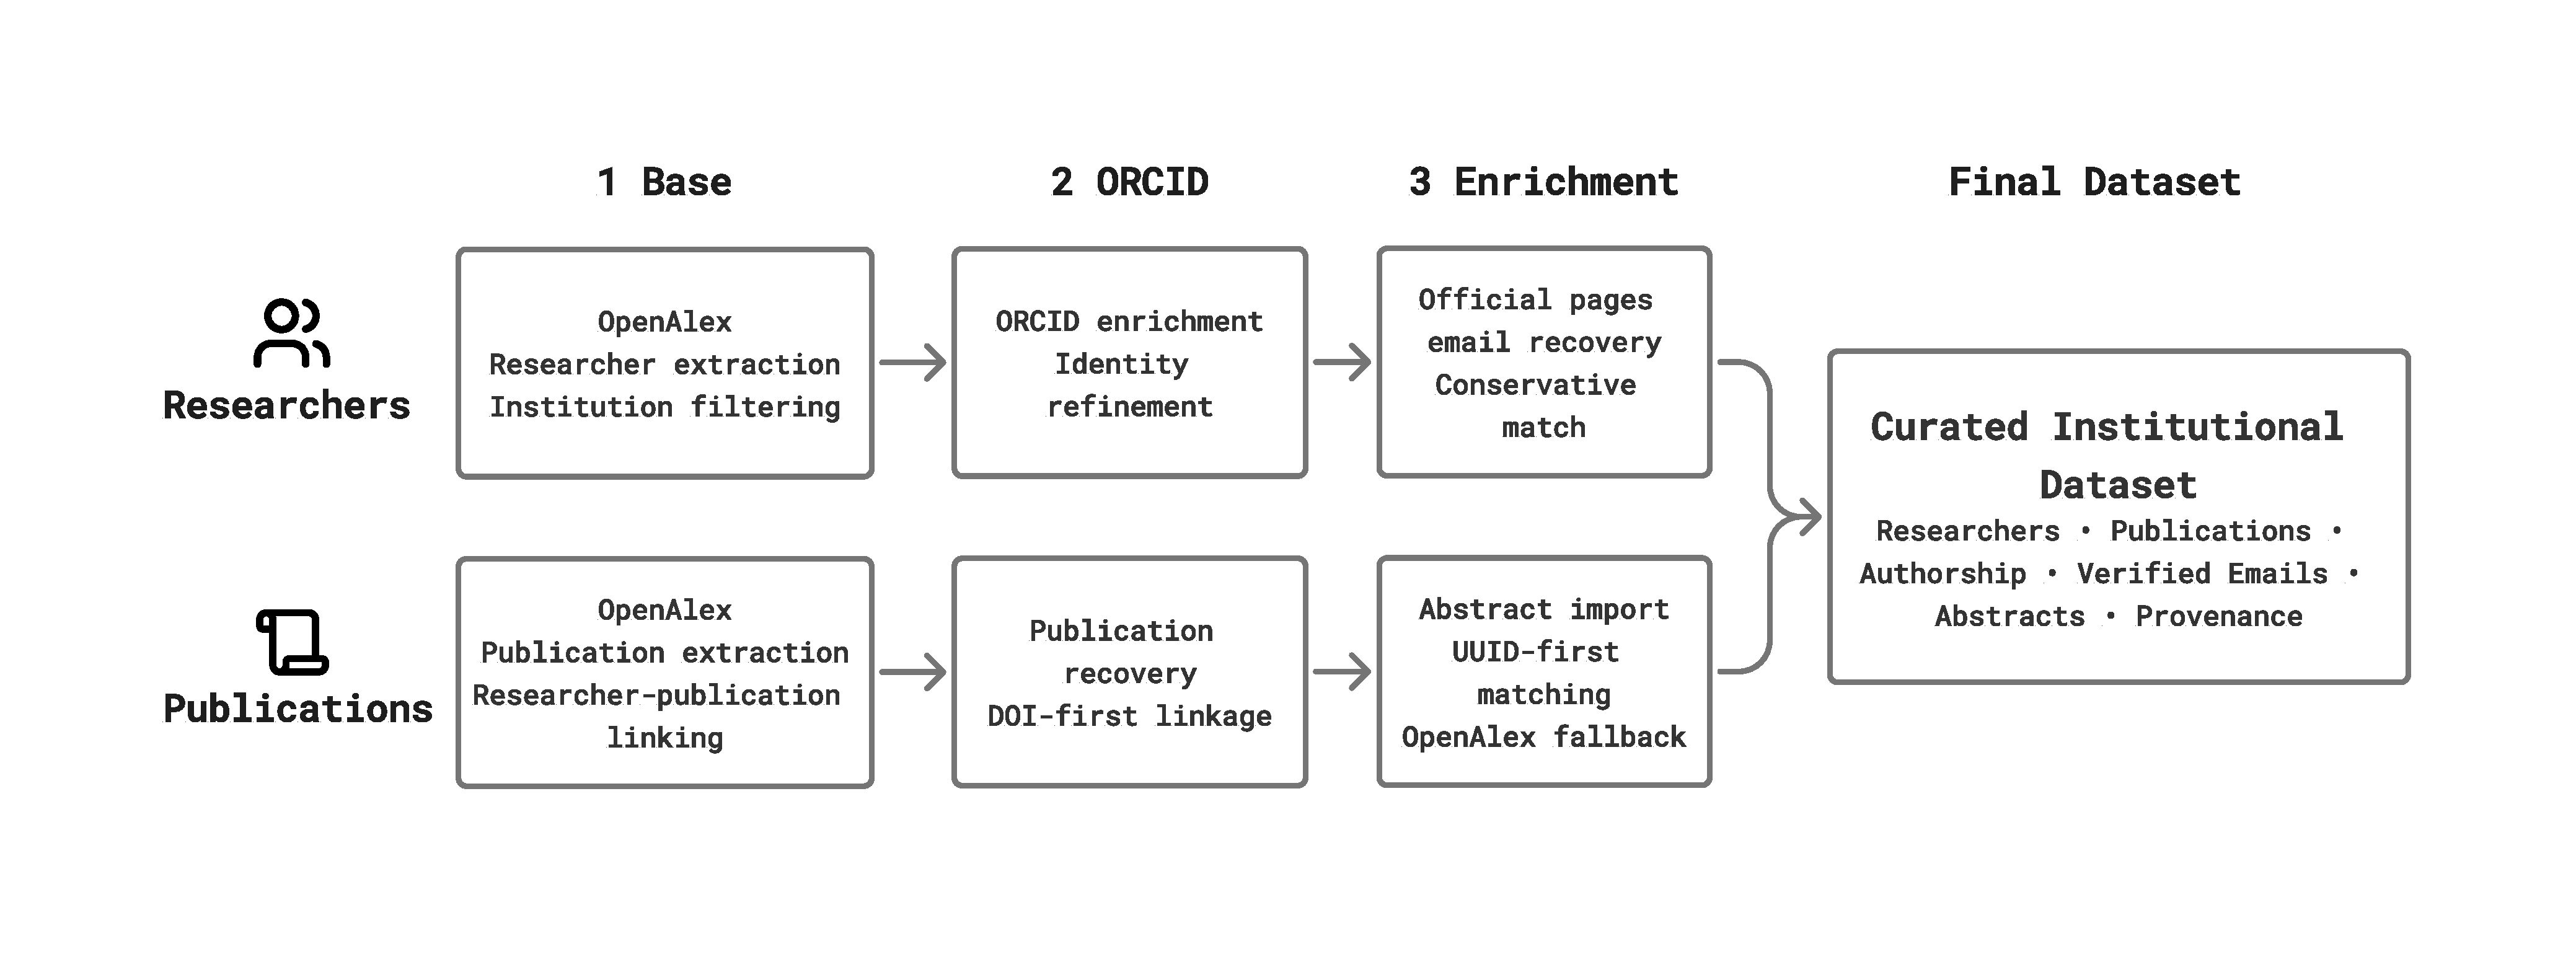
\includegraphics[width=\textwidth]{system_architecture.pdf}
\caption{Overview of the Unite! Researcher's Search data pipeline. OpenAlex serves as primary data source. Extracted researcher and paper entities are enriched through parallel pipelines before storage in the database.}
\label{fig:architecture}
\end{figure*}

\subsection{Data Collection and Integration}
%OpenAlex data for the nine universities served as the primary foundation of the dataset. We subsequently enriched these records using ORCID-linked researcher profiles, resulting in an approximately tenfold increase !!!z 600k do 2.9m, ewentualnie 5x!!! in the number of associated publications. Publication abstracts were then added through DOI-based matching, and contact email addresses were heuristically inferred and included where possible.
The dataset was constructed from OpenAlex using ROR-based institutional filters for the nine Unite! universities, yielding over 213,000 researcher profiles. These base records were subsequently enriched using public ORCID profiles, increasing publication coverage from 648,049 to nearly 3,000,000 records while supporting person-level disambiguation. Both researcher and publication counts continue to grow as additional data sources are integrated. Publication abstracts were then added through DOI-centered matching and auxiliary identifier-based reconciliation. Contact email addresses were incorporated through institution-specific recovery workflows, including heuristic methods where available.

\subsection{Entity Extraction and Enrichment}

The Entity Extraction and Enrichment phase transforms raw bibliographic records into a structured knowledge graph. The process is organized into two parallel pipelines targeting researchers and publications, respectively.

\subsubsection*{Researcher Pipeline}
The primary objective of this pipeline is to construct researcher profiles and link them to their published work.

\begin{itemize}
    \item \textbf{OpenAlex as Primary Source:} Researcher entities are initially sourced from the OpenAlex academic graph, which provides baseline profile data including names, institutional affiliations, and associated publication records.

    \item \textbf{ORCID Enrichment:} For researchers whose OpenAlex profiles contain an ORCID identifier---approximately 50\% of the dataset---the system queries the ORCID API to retrieve verified profile data, including confirmed affiliations and additional publication linkages. This step anchors researcher identities to a globally unique, author-controlled identifier, improving attribution accuracy. The remaining researchers without ORCID identifiers rely solely on OpenAlex metadata.
    \item \textbf{Heuristic Email Extraction:} As contact information is systematically absent from public academic datasets, the system implements a deterministic email synthesis algorithm. By combining parsed researcher name strings with institution-specific email domain patterns, the pipeline reconstructs probable contact addresses.
\end{itemize}
% jesli dopisanie nizszych sekcji nie naprawi formatowania: \raggedbottom
\subsubsection*{Publication Pipeline}

This pipeline improves the completeness, linkage quality and textual richness of publication records.
\begin{itemize}
    \item \textbf{OpenAlex Ingestion:} OpenAlex serves as the primary source for bulk publication metadata. Abstract ingestion involves programmatically reconstructing full text from OpenAlex's inverted index representation.

    \item \textbf{ORCID-Based Linkage:} For the subset of researchers with available ORCID identifiers, the system retrieves their publication lists directly from the ORCID API, forming higher-confidence author--paper linkages that complement the OpenAlex-derived associations.

    \item \textbf{DOI-Based Retrieval and Deduplication:} Digital Object Identifiers serve as the primary cross-source identifier for structural deduplication across the dataset. To address gaps in abstract coverage, an asynchronous pipeline queries the Crossref API using DOIs to retrieve missing abstracts. Retrieved data undergoes regex-based sanitization to strip JATS XML tags and HTML artifacts before batch insertion into the database. This enrichment pipeline has already increased total abstract coverage from 14.6\% to over 21\%, integrating approximately 190,000 previously missing abstracts.
\end{itemize}

\subsection{Search and Recommendation}
\label{sec:search}

The search subsystem operates in two complementary modes---semantic and keyword---unified through a hybrid ranking strategy.

\subsubsection*{Semantic Search}
Publication titles and abstracts are encoded into 1024-dimensional dense vector representations using BGE-M3 \cite{chen2024bgem3}, a multilingual embedding model that supports over 100 languages---a requirement given the linguistic diversity of the nine Unite! universities. Researcher-level embeddings are computed by averaging the vectors of all publications associated with a given author, producing a single representation that captures their aggregate research profile. Both publication and researcher embeddings are stored in a PostgreSQL database with the \texttt{pgvector} extension \cite{pgvector2024} and indexed using a Hierarchical Navigable Small World (HNSW) graph \cite{malkov2020hnsw} for approximate nearest neighbor retrieval. At query time, the user's free-text input is encoded with the same model and compared against stored embeddings via cosine similarity. This mode is particularly effective for exploratory queries where the user describes a research area in natural language rather than specifying exact technical terms.

\subsubsection*{Keyword Search}
For precise queries involving specific author names, method names, or technical vocabulary, the system supports full-text keyword search using PostgreSQL's built-in \texttt{tsvector} indexing with GIN indexes. Queries are parsed and matched against tokenized abstracts, titles, and researcher names with language-aware stemming and ranking via \texttt{ts\_rank}.

\subsubsection*{Hybrid Ranking}
When both search modes return results, the system combines them using Reciprocal Rank Fusion (RRF) \cite{cormack2009rrf}. Given ranked lists $R_{\text{sem}}$ and $R_{\text{kw}}$, each result $d$ receives a fused score:
\begin{equation}
\text{RRF}(d) = \sum_{r \in \{R_{\text{sem}},\, R_{\text{kw}}\}} \frac{1}{k + \text{rank}_r(d)}
\end{equation}
where $k=60$ is a smoothing constant. RRF is parameter-free beyond $k$ and robust to score scale differences between retrieval modes \cite{cormack2009rrf}. Results are re-ranked by fused score before presentation.

\subsubsection*{Filtering}
Users may constrain results by institution (any subset of the nine Unite! universities), publication year range, and research domain. Filters are applied as SQL predicates \emph{before} retrieval, ensuring that vector search operates over the filtered subset rather than post-filtering a global result set. This pre-filtering strategy preserves recall within the target scope while reducing query latency.

\subsubsection*{Query Assistance}
To reduce friction during interactive search, the system integrates Meilisearch \cite{meilisearch2024}, a search engine optimized for instant prefix matching and typo tolerance. As the user types, Meilisearch provides real-time autocompletion suggestions drawn from researcher names, publication titles, and topic labels indexed in the dataset. Its built-in typo-tolerance algorithm automatically corrects misspelled queries---particularly useful for non-native speakers searching for researcher names across multiple European languages. This component operates as a lightweight front-end layer: once the user selects or submits a query, it is forwarded to the hybrid retrieval pipeline described above.

\section{Demonstration}
\label{sec:demo}

The demonstration is designed as an interactive, live session in which attendees engage directly with \textsc{Unite! Researcher's Search} through a web-based interface. A supplementary video walkthrough of the full platform accompanies this paper. We structure the session around three progressively open-ended scenarios that showcase the system's core capabilities: cross-domain collaborator discovery, multi-source profile exploration, and audience-driven free-form search.

\subsection{Interface and Interaction}

The \textsc{Unite! Researcher's Search} interface presents a single search bar at the top of the page, accompanied by a filter panel that allows users to constrain results by institution, publication year range, and research domain. Upon submitting a query, the system returns a ranked list of researcher cards. Each card displays the researcher's name, primary institutional affiliation, a relevance-highlighted snippet from their most pertinent publication, total publication count, and---where available---a verified contact email. Clicking a card expands it into a full researcher profile view (described in Section~\ref{sec:scenario2}).

The interface supports both modes of search transparently: users may enter natural-language descriptions (e.g., ``machine learning for climate modeling'') for semantic search, or type specific names and technical terms for keyword-based retrieval. As the user types, real-time autocompletion suggestions and typo corrections appear below the search bar, helping users refine their queries before submission (Section~\ref{sec:search}). The system automatically selects the appropriate retrieval mode and combines results using hybrid ranking when both modes produce matches.

\subsection{Scenario 1: Discovering Collaborators}
\label{sec:scenario1}

In this scenario, the presenter demonstrates how \textsc{Unite! Researcher's Search} enables cross-domain collaborator discovery. The presenter types a research query such as ``graph neural networks for molecular property prediction'' into the search bar. The system returns a ranked list of researchers across multiple Unite! universities whose publication profiles are semantically related to the query. Importantly, the results may include researchers whose work is not described using identical terminology---for example, a computational chemist publishing on molecular representation learning---demonstrating the value of semantic search for bridging disciplinary vocabulary gaps.

For each result, the presenter highlights the enriched metadata: the researcher's ORCID-verified identity, their institutional affiliation, the number of matched publications, and the recovered contact email. The presenter contrasts this with a comparable query on OpenAlex or Google Scholar, where the same researcher's profile may be fragmented, lack contact information, or be absent from institution-filtered results entirely.

\subsection{Scenario 2: Exploring Researcher Profiles}
\label{sec:scenario2}

\begin{figure}[t]
\centering
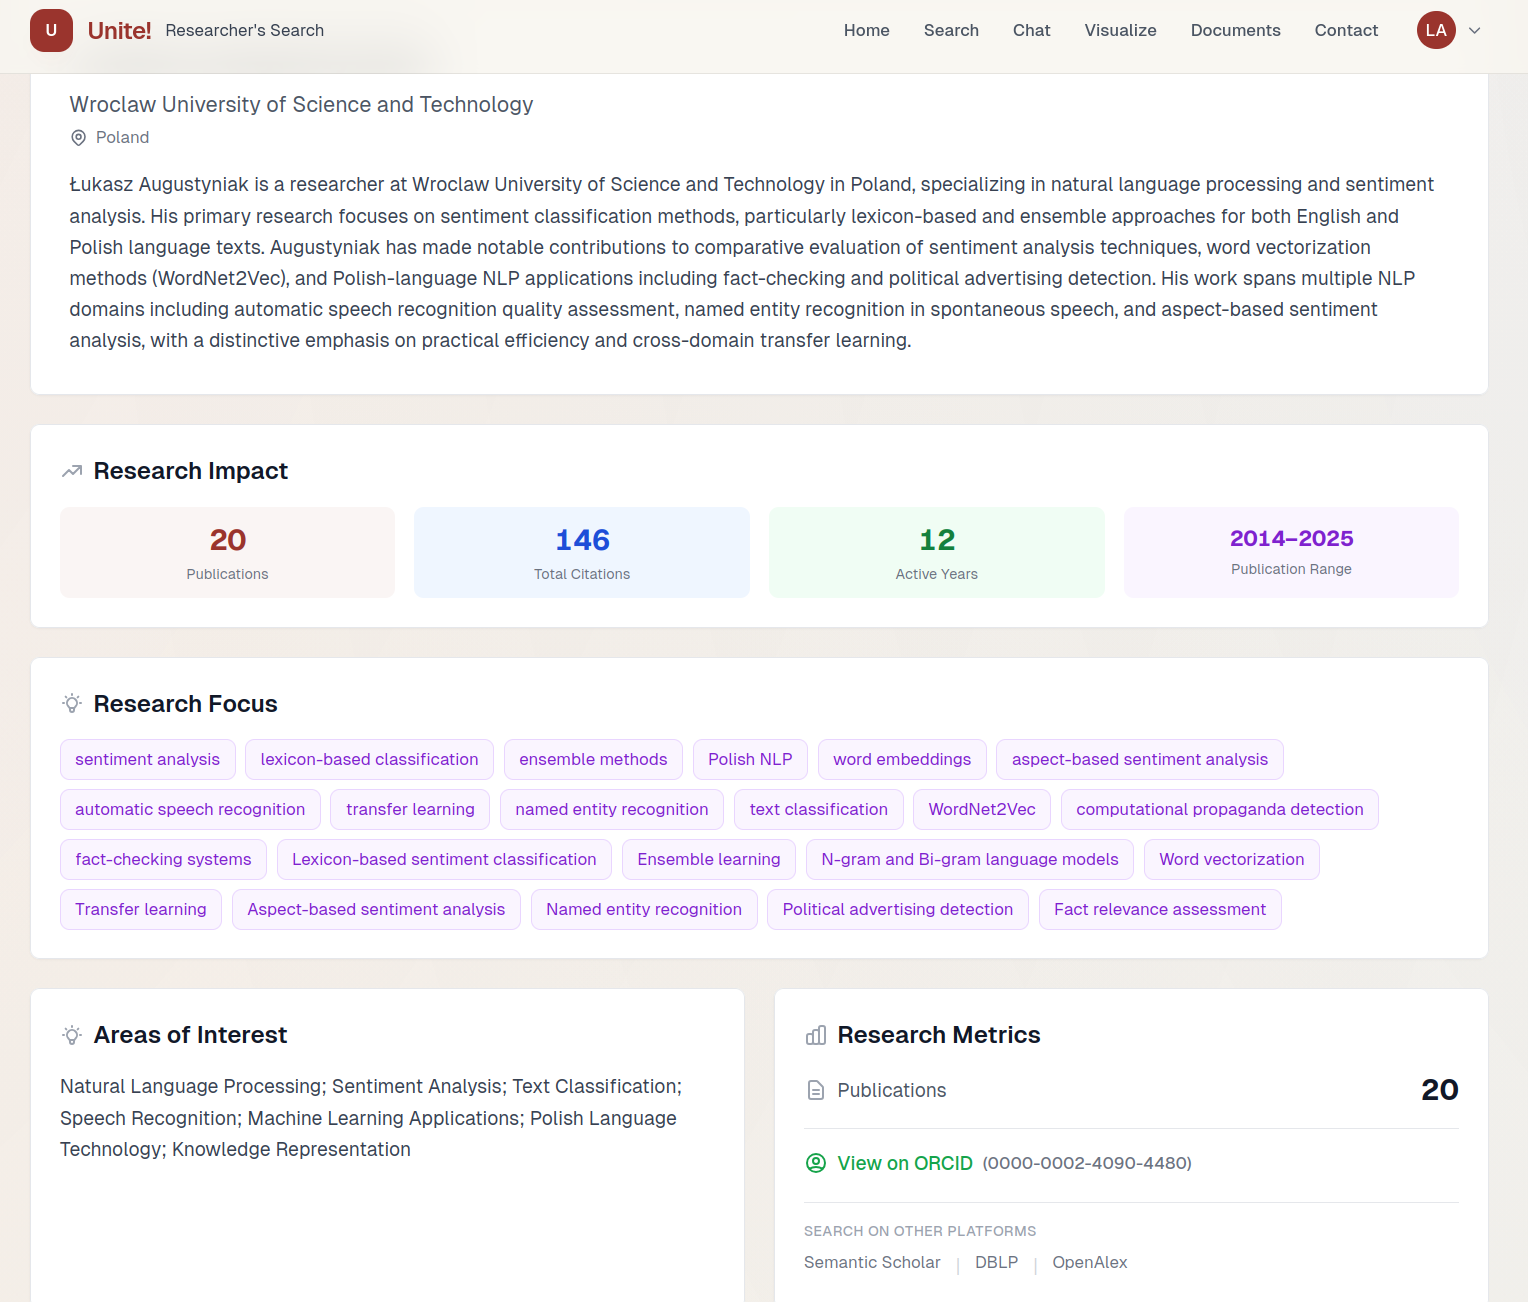
\includegraphics[width=\columnwidth]{figures/researcher-page.png}
\caption{Single researcher profile view. Information is aggregated from OpenAlex, ORCID, and Crossref; the biographical summary and research focus tags are semi-automatically generated.}
\label{fig:researcher-profile}
\end{figure}

The presenter selects a researcher from the Scenario~1 results and navigates to their full profile page (Figure~\ref{fig:researcher-profile}). The profile view demonstrates the practical impact of multi-source data fusion. Much of the displayed information is assembled from multiple complementary sources and, in several cases, semi-automatically generated. The profile presents:
\begin{itemize}
    \item \textbf{Identity and Contact:} Name, ORCID identifier, institutional affiliation sourced from OpenAlex and verified against ORCID records, and a recovered contact email.
    \item \textbf{Biographical Summary:} An automatically generated description of the researcher's expertise, synthesized from their publication history.
    \item \textbf{Research Impact and Focus:} Publication count, citations, active years, and automatically extracted topic labels and research area descriptors.
    \item \textbf{Cross-Platform Links:} Direct links to ORCID, Semantic Scholar, DBLP, and OpenAlex profiles for verification and further exploration.
\end{itemize}

The presenter shows how publications missing from a researcher's OpenAlex profile---but present in their ORCID record---appear in the unified view. Ongoing work focuses on automating periodic data refresh and improving quality assurance across the aggregation pipeline to keep profiles accurate as source databases evolve.

\subsection{Scenario 3: Audience-Driven Search}
\label{sec:scenario3}

In the final segment, attendees propose their own queries---searching for their own name to inspect how their profile has been constructed, or entering a research topic to discover relevant researchers across the network. This demonstrates robustness to unpredictable inputs and lets attendees evaluate semantic matching within their own expertise. The presenter moderates by collecting queries, executing them live, and discussing notable results such as unexpected cross-domain matches.

\section{Future Work}

Several directions remain for further development. First, we plan a systematic evaluation of hybrid retrieval, measuring latency, throughput, and ranking quality against expert judgments. Second, we intend to explore alternative researcher embedding strategies---such as recency-weighted or topic-clustered representations---to improve discriminability for prolific authors. Third, we aim to extend the platform beyond the nine Unite! universities to broader institutional networks.

\begin{acks}
This work was supported by the Department of Artificial Intelligence at Wroclaw University of Science and Technology.
\end{acks}

\bibliographystyle{ACM-Reference-Format}
\bibliography{bibiliography}

\end{document}
\endinput
